\documentclass[10pt]{article}
\usepackage[utf8]{inputenc}
\usepackage{geometry}
\usepackage[sort]{natbib}
\usepackage{pxfonts}
\usepackage{graphicx}
\usepackage{setspace}
\usepackage{hyperref}
\usepackage{lineno}
\usepackage{authblk}
\usepackage{pdflscape}
\usepackage{rotating}

\doublespacing
\linenumbers

\title{\textit{Supplementary materials for:} Fitness tracking reveals task-specific associations between
  memory, mental health, and exercise}
\author[1, $\star$]{Jeremy R. Manning}
\author[1,2]{Gina M. Notaro}
\author[1]{Esme Chen}
\author[1]{Paxton C. Fitzpatrick}
\affil[1]{Dartmouth College, Hanover, NH}
\affil[2]{Lockheed Martin, Bethesda, MD}
\affil[$\star$]{Address correspondence to jeremy.r.manning@dartmouth.edu}

\newcommand{\task}{1}
\newcommand{\immediateBehavior}{2}
\newcommand{\delayedBehavior}{3}
\newcommand{\fitness}{4}
\newcommand{\MHcorr}{5}
\newcommand{\dynamics}{6}


\begin{document}
\maketitle

\renewcommand{\thefigure}{S\arabic{figure}}


\begin{figure}[p]
\centering
\includegraphics[width=0.6\textwidth]{figs/devices}
\caption{\textbf{Fitbit devices.}  The bars indicate the numbers of
  participants whose fitness tracking data came from each model of
  Fitbit device.  ``MobileTrack'' refers to participants who used
  smartphone accelerometer information to track their activity via the
  Fitbit smartphone app.
  ``Unknown''  denotes participants whose device information was not
  available from their available Fitbit data.}
\label{fig:devices}
\end{figure}


\begin{sidewaysfigure}[p]
\centering
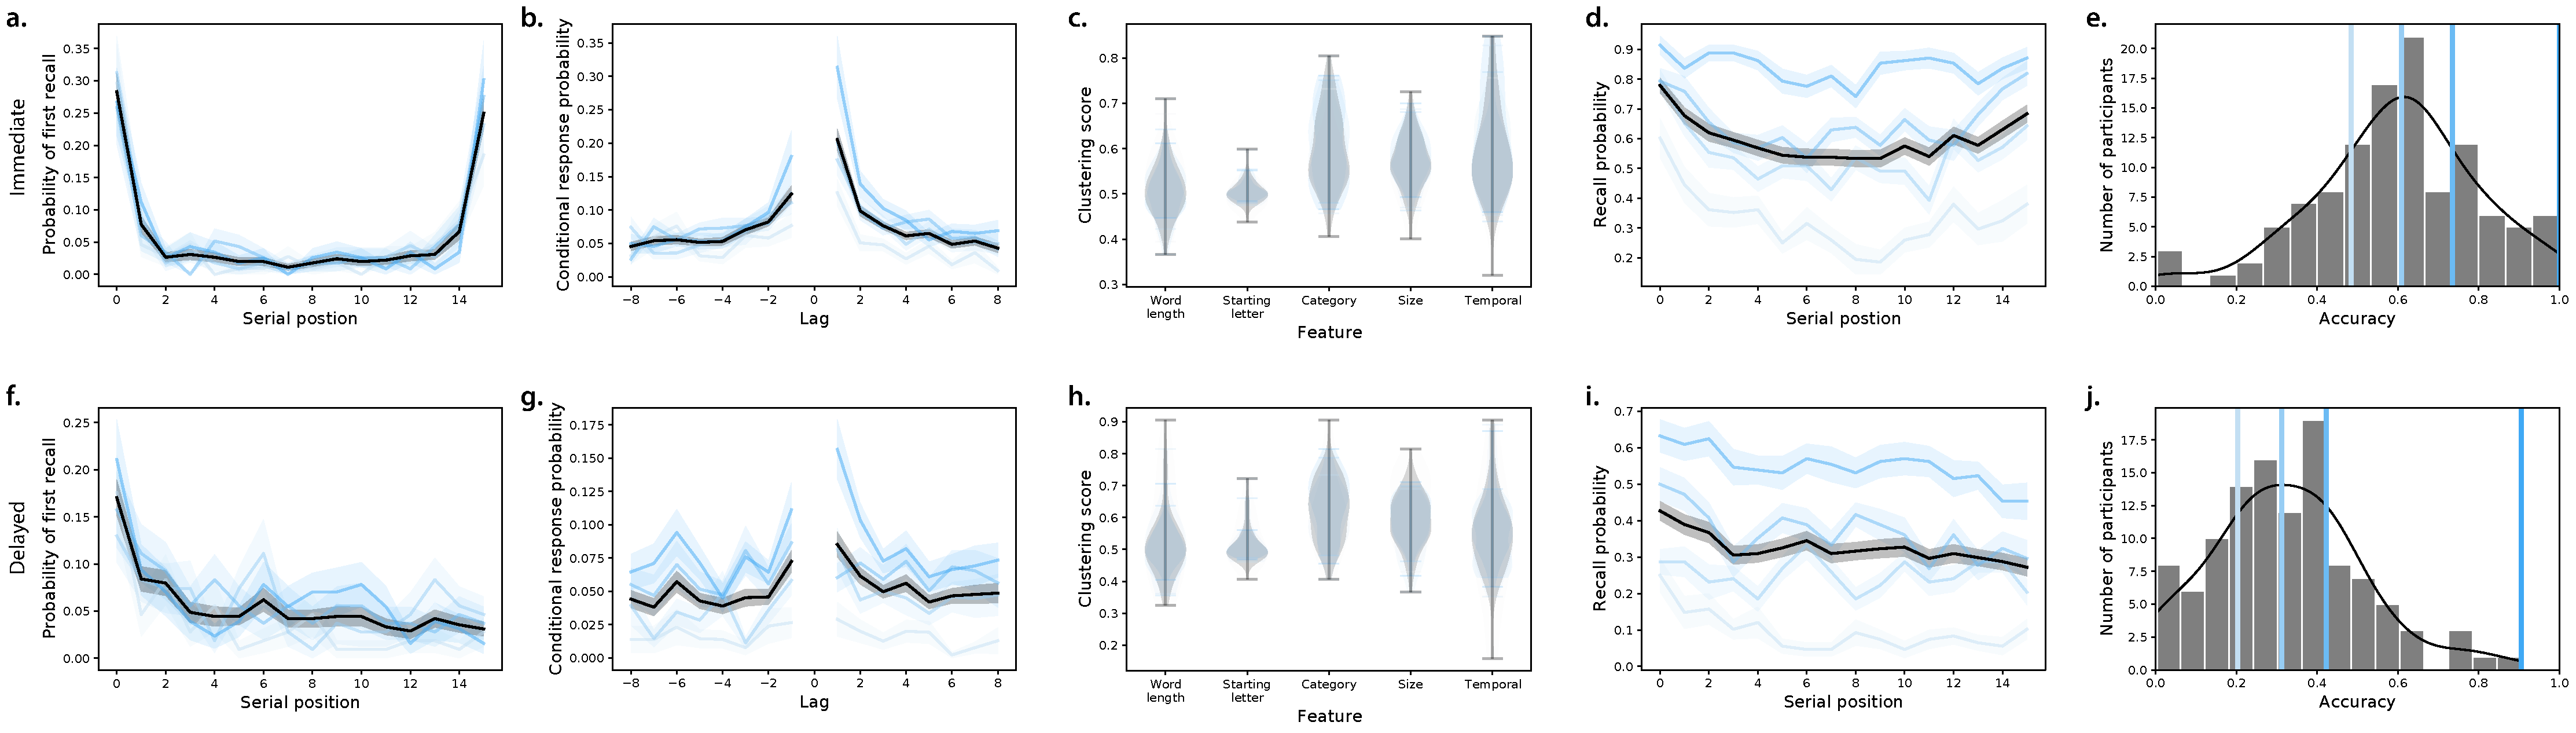
\includegraphics[width=1\textwidth]{figs/free_recall_behavior}
\caption{\textbf{Free recall behavioral results.  a--e. Immediate free
  recall.}  \textbf{a. Probability of first recall.}  Probability of
recalling each studied word first, as a function of its presentation
position.  \textbf{b. Lag Conditional Response Probability.}
Probability of recalling the word presented at position $i +
\mathrm{Lag}$ following the recall of the word presented at position
$i$.  \textbf{c. Clustering scores.}  Each score denotes participants'
tendancies to successively recall (cluster) words according to the
given feature dimension~\citep{PolyEtal09}: word length, starting letter, (semantic)
category, size (large or small), or presentation position (temporal).
\textbf{d. Serial position curve.}  Probability of recalling each word
as a function of its presentation position.  \textbf{e. Recall
  accuracy.}  Distribution of the average proportions of recalled
words, across all lists studied by each participant.  \textbf{f--j.
  Delayed free recall.}  These panels are in the same formats as
Panels a -- e, but they reflect performance on the delayed free recall
memory tests.  All panels: error bars and error ribbons denote bootstrap-estimated
95\% confidence intervals.  Shading (saturation) denotes results for
different subsets of participants, according to the average
proporition of words they remembered (group boundaries are indicated
by the colored lines in Panels e and j).}
\label{fig:fr_behavioral}
\end{sidewaysfigure}

\begin{sidewaysfigure}[p]
\centering
\includegraphics[width=1\textwidth]{figs/naturalistic_recall_behavior}
\caption{\textbf{Naturalistic recall behavioral results.}
  \textbf{a. Identified topics.}  Applying a topic model to a series
  of sliding windows of the video's transcript~\citep{HeusEtal21}
  revealed a set of 13 unique (non-trivial) topics.  The Panel
  displays the 5 top-weighted words from each topic.  \textbf{b. Topic
  timecourse of the video.}  Each row displays the topic weights for a
single moment of the video.  \textbf{c. Topic correlation matrix.}  The
correlations between the topic vectors for each pair of moments from
the video reveals an event-like block diagonal structure.
\textbf{d. Video topic trajectory.}  The topic video's topic
timecourse (Panel b) has been projected onto 2-dimensions using
Uniform Manifold Approximation and
Projection~\citep[UMAP;][]{McInEtal18}.  Each colored dot reflects an
event, identified by applying a Hidden Markov Model to the video's
topic timecourse~\citep{BaldEtal17, HeusEtal21}.  Red dots denote
earlier timepoints in the video and blue dots denote later
timepoints.  \textbf{e. Immediate recall trajectory.}  The black curve
displays the average
topic timecourse (projected into 2D using UMAP), obtained by applying the topic model shown in Panel A
to the participants' written transcripts from the immediate recall
test.  The arrows denote agreement across participants in the
directions of their topic trajectories, for participants whose
trajectories intersected the corresponding region of topic space.
Blue arrows denote reliable agreement across participants ($p < 0.05$, corrected).
\textbf{f. Delayed recall trajectory.} This panel is in the same
format as Panel e, but displays the trajectory for participants'
delayed recall of the video.  \textbf{g. Immediate recall precision.}  Distribution of
average recall \textit{precision}, across all of the events each
participant recalled during the immediate recall test.  Precision is
defined as the correlation between the topic vector for a given
recalled event and the best-matching (most highly correlated) video
event's topic
vector~\citep{HeusEtal21}.  \textbf{h. Delayed recall precision.}
This panel is in the same format as Panel g, but displays the average
precision values for the delayed memory test.}
\label{fig:nat_behavioral}
\end{sidewaysfigure}

\begin{figure}[p]
\centering
\includegraphics[width=0.6\textwidth]{figs/vocab_learning_behavior}
\caption{\textbf{Foreign language vocabulary learning behavioral
    results.}  \textbf{a. Immediate recall.}  Average proportions of
  correctly identified Gaelic-English word pairs from \textit{early} (first 3) and
\textit{late} (last 3) study positions, or aggregated over
\textit{all} study positions.  \textbf{b. Distribution of proportion
  of correctly recalled pairs on the immediate memory test.}  The colored
lines indicate quartile boundaries, and correspond to the coloring in
Panel a.  Note that the right-most edge of the third quartile overlaps
with the top quartile, since over 25\% of the participants correctly recalled
90\% of the word pairs correctly, but no participant achieved 100\%
accuracy.  \textbf{c--d. Delayed recall.}  These panels are in the
same formats as Panels a and b, but reflect performance on the delayed
recall test.  The error bars in Panels a and c denote
bootstrap-estimated 95\% confidence intervals.}
\label{fig:vocab_behavioral}
\end{figure}

\begin{figure}[p]
\centering
\includegraphics[width=0.6\textwidth]{figs/spatial_learning_behavior}
\caption{\textbf{Spatial learning behavioral results.}}
\label{fig:spatial_behavioral}
\end{figure}

\begin{sidewaysfigure}[p]
\centering
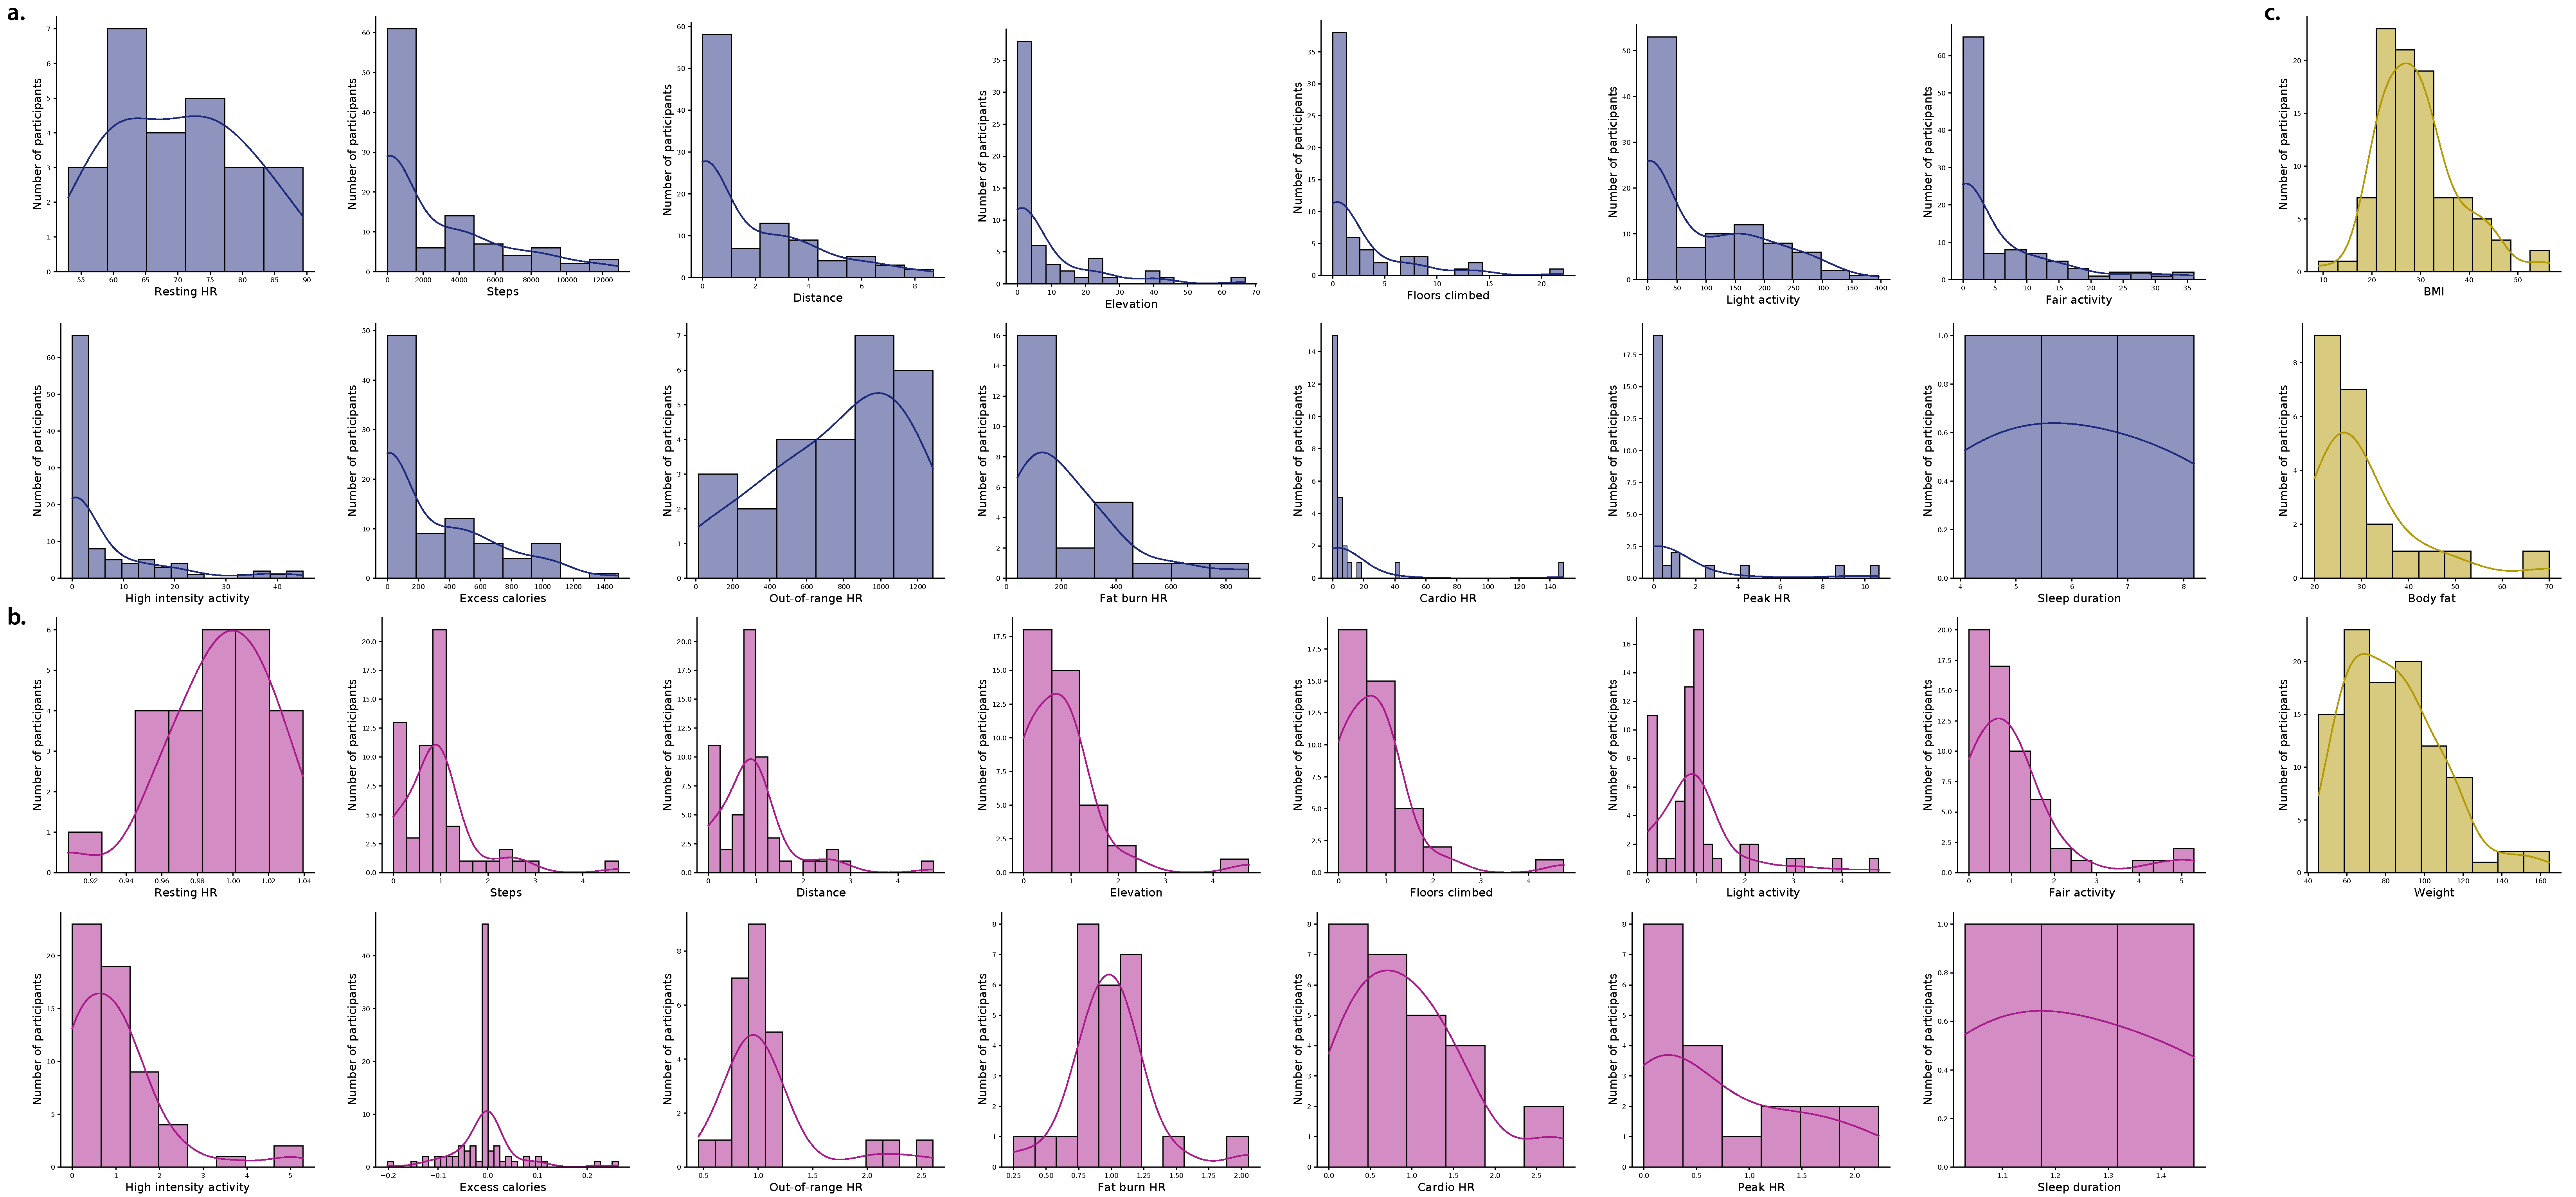
\includegraphics[width=\textwidth]{figs/fitness_distributions}
\caption{\textbf{Distributions of fitness measures.}}
\label{fig:fitness_dists}
\end{sidewaysfigure}

\begin{sidewaysfigure}[p]
\centering
\includegraphics[width=\textwidth]{figs/fitness_dists_immediate}
\caption{\textbf{Distributions of fitness measures, broken down
    by immediate task performance.}}
\label{fig:fitness_dists_immediate}
\end{sidewaysfigure}

\begin{sidewaysfigure}[p]
\centering
\includegraphics[width=\textwidth]{figs/fitness_scatter_immediate}
\caption{\textbf{Scatterplots of fitness measures versus
    immediate task performance measures.}}
\label{fig:fitness_scatters_immediate}
\end{sidewaysfigure}

\begin{sidewaysfigure}[p]
\centering
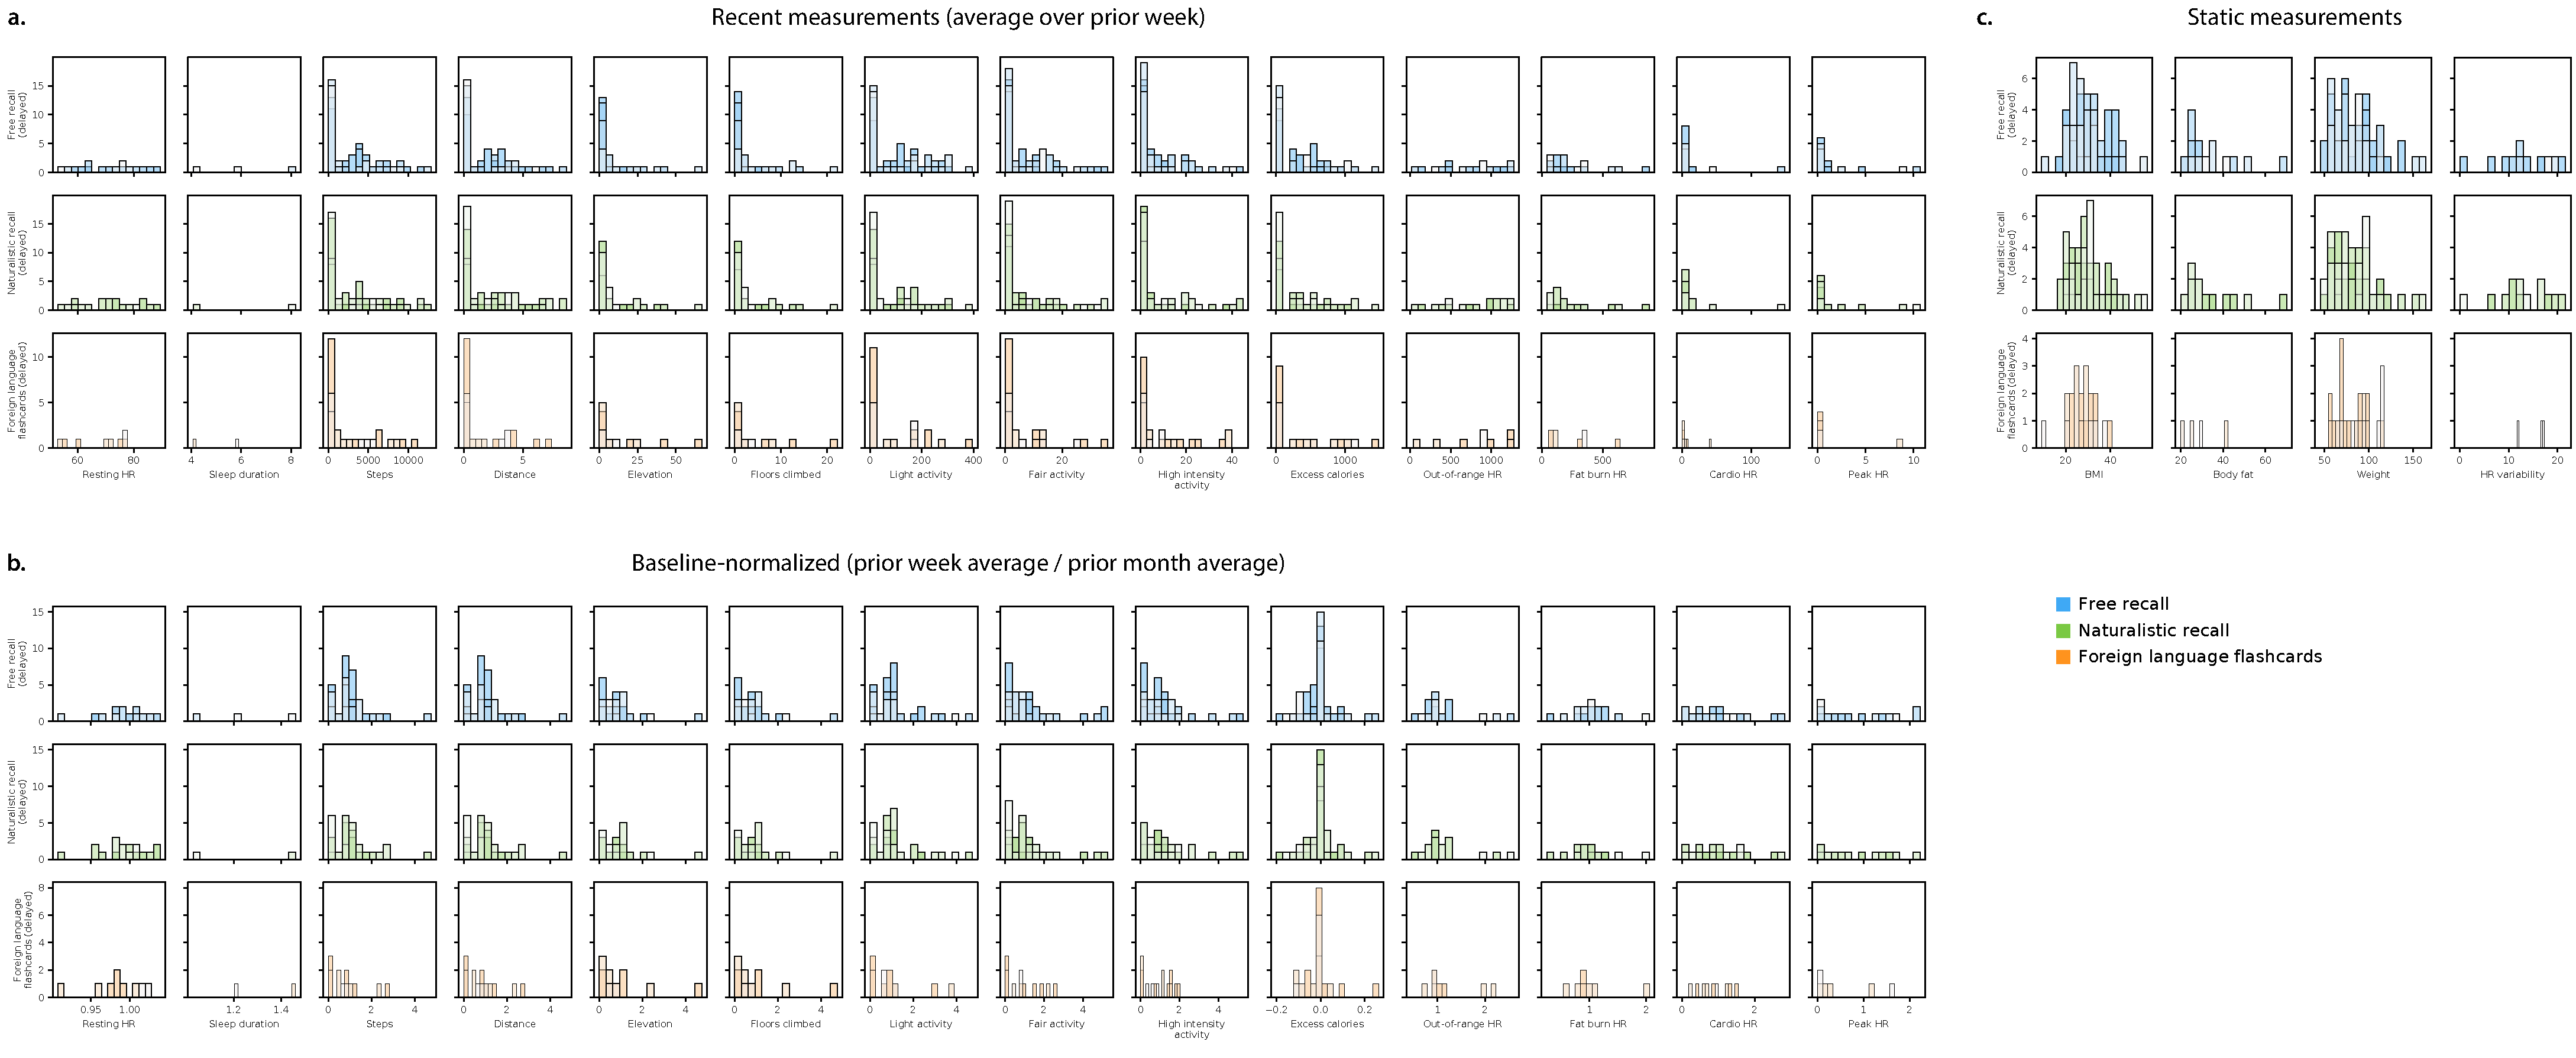
\includegraphics[width=\textwidth]{figs/fitness_dists_delayed}
\caption{\textbf{Distributions of fitness measures, broken down
    by delayed task performance.}}
\label{fig:fitness_dists_delayed}
\end{sidewaysfigure}

\begin{sidewaysfigure}[p]
\centering
\includegraphics[width=\textwidth]{figs/fitness_scatter_delayed}
\caption{\textbf{Scatterplots of fitness measures versus
    delayed task performance measures.}}
\label{fig:fitness_scatters_delayed}
\end{sidewaysfigure}

\begin{figure}[p]
\centering
\includegraphics[width=0.4\textwidth]{figs/behavior_behavior_correlations}
\caption{\textbf{Bootstrap-estimated reliable correlations between
    behavioral measures.}}
\label{fig:behavioral_corrs}
\end{figure}

\begin{figure}[p]
\centering
\includegraphics[width=\textwidth]{figs/fitness_fitness_correlations}
\caption{\textbf{Bootstrap-estimated reliable correlations between
    fitness measures.}}
\label{fig:fitness_corrs}
\end{figure}

\begin{figure}[p]
\centering
\includegraphics[width=\textwidth]{figs/survey_survey_correlations}
\caption{\textbf{Bootstrap-estimated reliable correlations between
    demographic measures.}}
\label{fig:survey_corrs}
\end{figure}

\begin{sidewaysfigure}[p]
\centering
\includegraphics[width=\textwidth]{figs/behavior_fitness+survey_correlations}
\caption{\textbf{Bootstrap-estimated reliable correlations between
    behavioral measures and fitness or demographic measures.}}
\label{fig:fitness_survey_corrs}
\end{sidewaysfigure}

\begin{figure}[p]
  \centering
  \includegraphics[width=0.75\textwidth]{figs/weighted_timecourse_activity}
\caption{\textbf{History of fitness activity levels weighted by
    behavioral performance.}}
\label{fig:activity_timecourse}
\end{figure}

\begin{figure}[p]
  \centering
  \includegraphics[width=0.7\textwidth]{figs/weighted_timecourse_HR}
\caption{\textbf{History of cardiovascular activity weighted by
    behavioral performance.}}
\label{fig:HR_timecourse}
  \end{figure}

\begin{figure}[p]
  \centering
  \includegraphics[width=0.75\textwidth]{figs/weighted_timecourse_sleep}
\caption{\textbf{History of sleep efficiency and duration weighted by
    behavioral performance.}}
\label{fig:sleep_timecourse}
\end{figure}

\begin{sidewaysfigure}[p]
  \centering
  \includegraphics[width=0.75\textwidth]{figs/weighted_timecourse_activity_MH}
\caption{\textbf{History of fitness activity levels weighted by
    mental health factors.}}
\label{fig:activity_timecourse_MH}
\end{sidewaysfigure}

\begin{sidewaysfigure}[p]
  \centering
  \includegraphics[width=\textwidth]{figs/weighted_timecourse_HR_MH}
\caption{\textbf{History of cardiovascular activity weighted by
    mental health factors.}}
\label{fig:HR_timecourse_MH}
  \end{sidewaysfigure}

\begin{figure}[p]
  \centering
  \includegraphics[width=0.75\textwidth]{figs/weighted_timecourse_sleep_MH}
\caption{\textbf{History of sleep efficiency and duration weighted by
    mental health factors.}}
\label{fig:sleep_timecourse_MH}
  \end{figure}

  \clearpage
  \newpage
\bibliographystyle{apa}
\bibliography{/Users/jmanning/CDL-bibliography/cdl}
\end{document}
